\section{Bảy lượt kiểm tra hội tụ muộn trên PVSG}\label{app:late}
Mỗi hàng đối chiếu hai lượt có cùng mô hình và seed. Lượt gốc có cả hai
recall test bằng 0. Khi hoãn thời điểm được phép dừng, cả bảy lượt vẫn có
recall validation bằng 0 đến hết epoch 16. Lượt trúng validation đầu tiên
xuất hiện trong khoảng epoch 17--20. Bảng~\ref{tab:late} ghi kết quả test
của checkpoint chọn bằng validation trong mỗi lượt kiểm tra bổ sung.
\begin{table}[H]\centering\small
\caption{Kết quả từng seed khi hoãn early stopping. Đơn vị \%.}\label{tab:late}
\begin{tabular}{@{}lrrr@{}}\toprule
Cấu hình ST-GAT & Seed & R@50 & mR@50\\\midrule
Đầy đủ & 17 & 5,26 & 1,87\\
Đầy đủ & 2026 & 4,73 & 2,31\\
Bỏ cạnh thời gian & 17 & 4,83 & 1,77\\
Bỏ cạnh thời gian & 2026 & 2,15 & 0,41\\
Chỉ giữ self-loop & 17 & 3,76 & 1,52\\
Chỉ giữ self-loop & 42 & 3,65 & 1,55\\
Chỉ giữ self-loop & 2026 & 3,44 & 1,46\\
\bottomrule\end{tabular}
\end{table}
\section{Ví dụ thời gian trên track chuẩn}
\begin{figure}[H]\centering
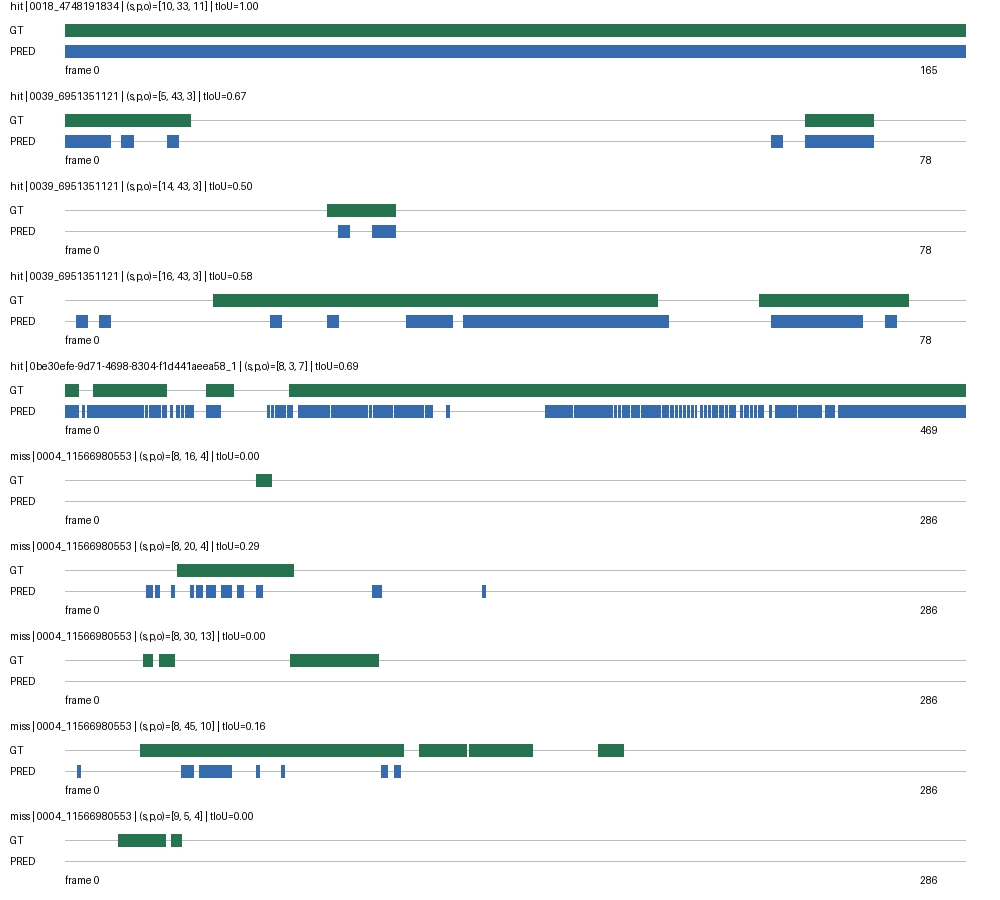
\includegraphics[width=.80\linewidth]{case_timelines.png}
\caption{Đoạn chuẩn (GT, xanh lá) và đoạn dự đoán (PRED, xanh dương) của Static GAT seed 17. Mười trường
hợp được lấy theo thứ tự video và bộ ba trong mỗi nhóm trúng hoặc bỏ sót.
Mỗi hàng có trục frame riêng.}\label{fig:timeline}
\end{figure}
